\documentclass[./main_en.tex]{subfiles}
\graphicspath{{\subfix{./figs}}}

% ------------ main document ------------
\begin{document}
\nolinenumbers

% style setup
\newpage
\renewcommand{\headrulewidth}{0pt}
\thispagestyle{fancy}
%... then configure it
\fancyhf{} % Clear all header and footer fields.
\fancyfoot{} % clear all footer fields
\fancyfoot[C]{\thepage}

\par \hfill
\vspace{40mm}
\begin{adjustwidth}{45pt}{45pt}
\begin{center}
    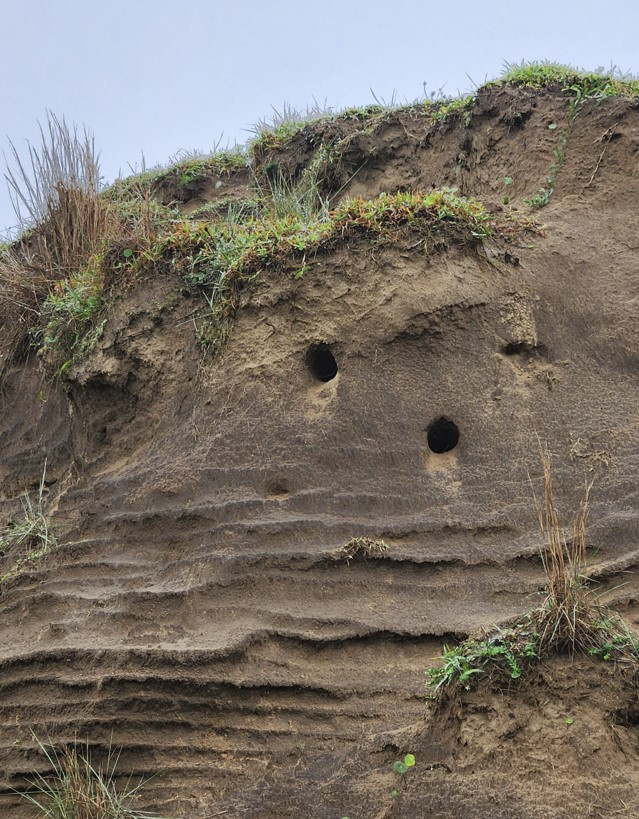
\includegraphics[scale=0.7]{figs/fig_tucos.jpg}\\
\end{center}
\vspace{10mm}
\noindent \textsf{The soil mantle acts as a natural reservoir for rainwater, storing it in its internal cavities. The fauna and flora, by excavating macropores, not only create pathways for water infiltration but also accelerate its release, especially in the upper horizons.}
\end{adjustwidth}
\clearpage
\end{document}